\subsection{Implicit model: Solvation Free Energy}

Solvation is the process of reorganizing solvent and solute molecules into solvation systems. Solvation involves bond formation, hydrogen bonding, and van der Waals forces. Solvation of a solute by water is called hydration \cite{campbell2006chemistry}. The solvation process describes the interaction between the solute and solvent molecules. This process will be thermodynamically favored only if the overall Gibbs energy of the solution is decreased, compared to the Gibbs energy of the separated solvent and solid (or gas or liquid). Regarding Equation \ref{eq:Gibbs}, a negative Gibbs energy indicates a spontaneous process but does not provide information about the rate of dissolution.

This process involves multiple steps with different energy consequences: First, a cavity must form in the solvent to make space for a solute (Figure \ref{fig:solv_1} to Figure \ref{fig:solv_2}). This is both entropically and enthalpically unfavorable, as solvent ordering increases and solvent-solvent interactions decrease. Stronger interactions among solvent molecules leads to a greater enthalpic penalty for cavity formation. Next, a particle of solute must separate from the bulk. This is enthalpically unfavorable since solute-solute interactions decrease, but when the solute particle enters the cavity, the resulting solvent-solute interactions are enthalpically favorable. 

\begin{figure}[h]
    \centering
    \begin{subfigure}[t]{0.25\textwidth}
    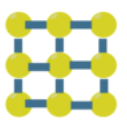
\includegraphics[width=\textwidth]{Figures/Chapter 4/Cavity_1.png}
    \caption{Representation of bulk solvent.}
    \label{fig:solv_1}
    \end{subfigure}
    \hspace{0.5cm}
    \begin{subfigure}[t]{0.25\textwidth}
    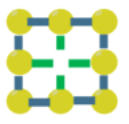
\includegraphics[width=\textwidth]{Figures/Chapter 4/Cavity_2.png}
    \caption{A cavity with the solute geometry is form in the solvent.}
    \label{fig:solv_2}
    \end{subfigure}
    \hspace{0.5cm}
    \begin{subfigure}[t]{0.25\textwidth}
    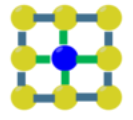
\includegraphics[width=\textwidth]{Figures/Chapter 4/Cavity_3.png}
    \caption{The solute is placed in the solvent cavity with the respective solute-solvent interactions}
    \label{fig:solv_3}
    \end{subfigure}
   
    \caption{Representation of the solvation process for any molecule in solution.}
    \label{fig:solvation}
\end{figure}
The solvation free energy, process described in Figure \ref{fig:solvation}, is frequently decomposed as a sum of \textit{polar} $(\Delta G_{polar})$ and \textit{non-polar} $(\Delta G_{np})$ terms  \cite{zacharias2003continuum}. 
\begin{equation}
    \Delta G^{solv} = \Delta G_{polar}^{solv} + \Delta G_{np}^{solv}
    \label{eq:G_solv}
\end{equation}
The polar term is the free energy of creating the solute’s charge distribution inside a pre-existing solute cavity, Assuming a charge distribution given by a molecular mechanics force field, the polar solvation contribution can be modeled with macroscopic continuum dielectric theory, e.g. the Poisson-Boltzmann equation. This works focuses on the \textbf{non-polar} component which is define as the work required to place an uncharged solute inside the solvent and generates a dry cavity on it. This contribution is often estimated from the solvent accessible surface area (SASA) of the molecule using a uniform surface tension coefficient obtained from a fit of experimental \cite{zacharias2003continuum}. 

\subsubsection{Solvent-Accessible Surface Area (SASA) Model}\label{subsubsec:SASA_model}
Implicit-solvent models often treat $\Delta G_{np}$ as a weighted combination of the solute’s SASA and other geometric measures given by: 
\begin{equation}
    \Delta G_{np} = \gamma (SASA) + b
    \label{eq:SASA}
\end{equation}
where $\gamma$ is is usually interpreted as the liquid-vapor surface tension, and $b$ is a scaling constant. Geometrically, \textit{Solvent Accessible Surface Area} is related to the region of the molecule surface exposed enough to be able to interact with solvent molecules. It is usually defined as a surface built by the delineation drawn by the center of a sphere (rough representation of a solvent molecule, usually of 1.4 [\r{A}] radii; i.e. a water molecule) rolling over the molecular surface. 
Nevertheless, the accurate prediction of the solvation free energy remains a very challenging issue and several inaccuracies with this method have been presented by some authors \cite{gallicchio2000enthalpy} \cite{wang2018breaking},  suggesting that an empirical parametrization of the hydration free energy and the free energy of association of apolar species based only on the solvent accessible surface area is insufficient. Successful parametrization should contain a surface area term to reproduce effects due to entropy loss and solvent reorganization energy and terms that depend on the number, location, and type of atomic interaction centers to reproduce effects due to the solute-solvent dispersion interactions which are only weakly correlated with surface area. 









